\clearpage
\subsection{T5 + PICARD} \label{picard}

\subsubsection{T5 + PICARD} \label{picard}

% \begin{figure}[H]
%     \centering
%     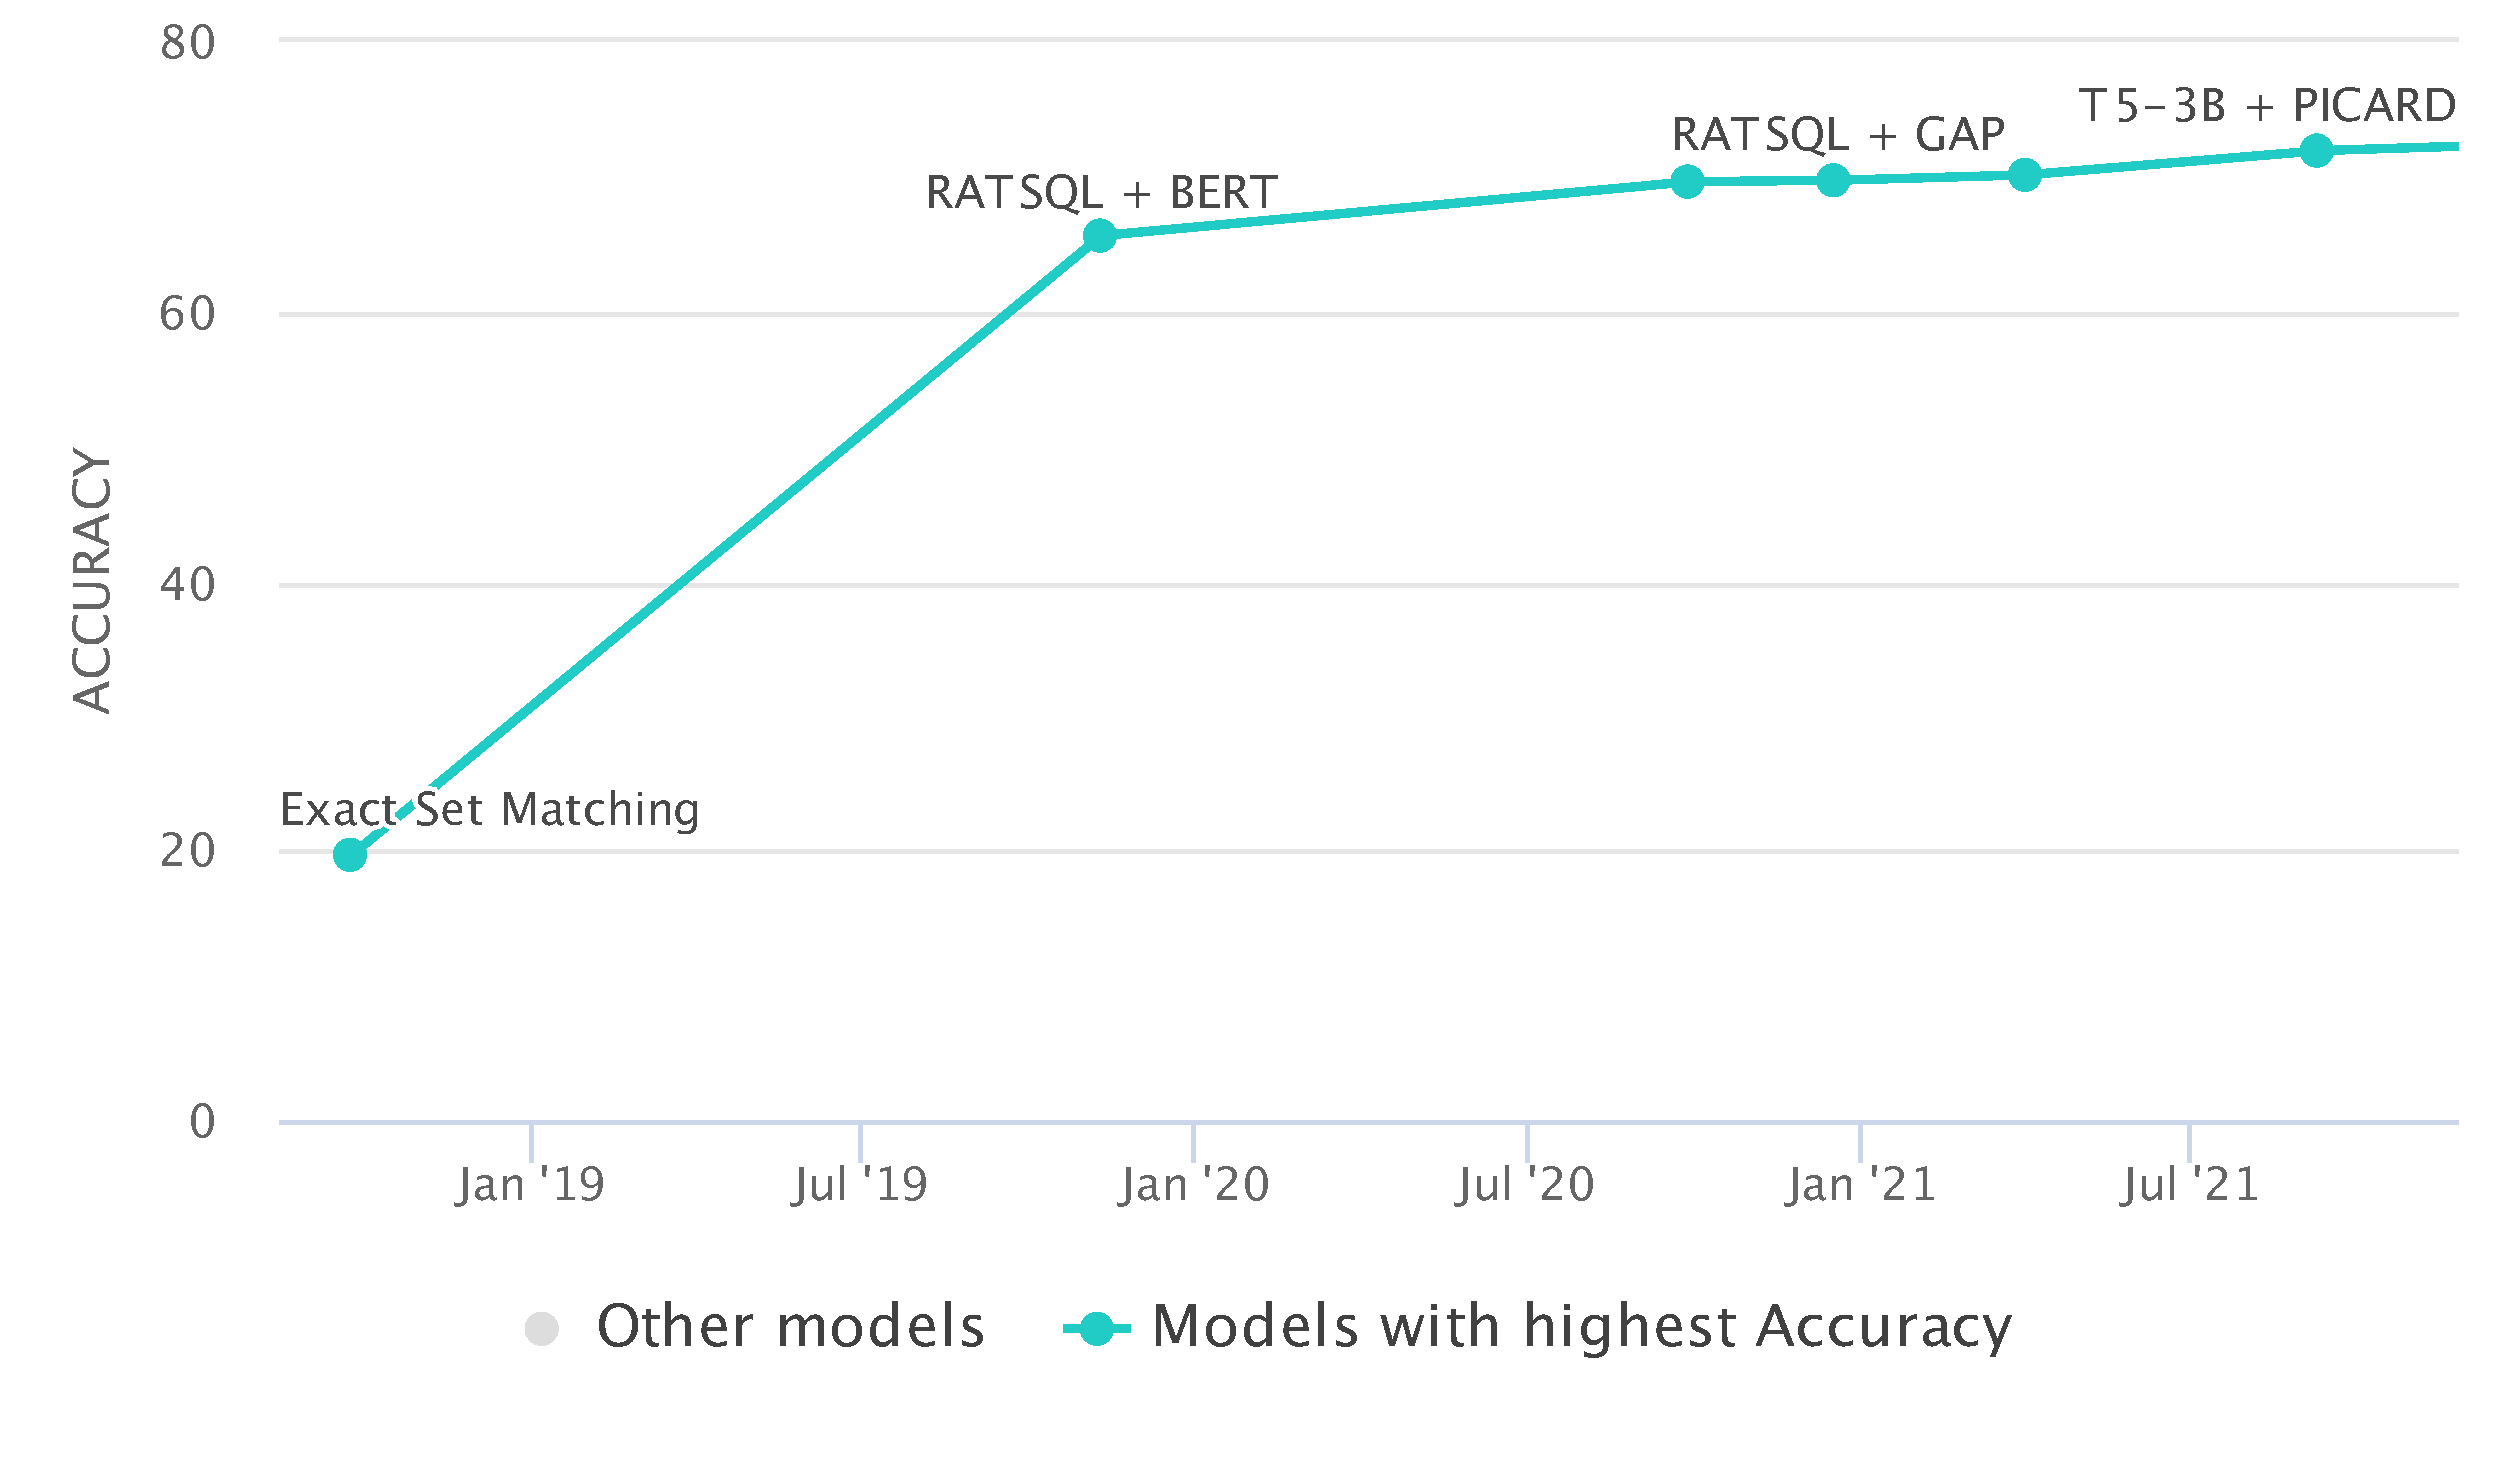
\includegraphics[page=1,width=0.7\textwidth]{pics/picard/benchmark.pdf}
%     \caption{Benchmark results for the PICARD model\cite{picard2020picard}}
% \end{figure}

After the release of Google T5, researchers have been using it to improve the accuracy of text-to-SQL models instead of BERT. New solutions have been released, such as the PICARD with T5-3B model, that significantly improved the SPIDER challenge's accuracy and are motivating researchers to use T5 in their work with innovative approaches since 2021.

\subsubsection*{T5}

In Transfer Learning, we start by training our model in an unsupervised fashion on unlabeled data. Then fine-tuning it on a labeled dataset some tasks that we care about, which we call the downstream tasks. For instance, in our unsupervised free training task, we take some text, drop out some of the words, and train the model to predict the missing words. Next, we will fine-tune it on a supervised task like sentiment analysis classifying movie reviews as a given label. This way of training has become an incredible recipe for natural language processing.

\ac{T5} Model implemented by Raffel et al. \cite{raffel_exploring_2020} uses the BERT encoder-decoder architecture proposed by Vaswani et al. (2017){devlin-etal-2019-bert} and they showed in their studies that it will outperform decoder-only language models. Originally T5 was introduced with five pre-trained models — Small (60 million parameters), Base(220 million parameters), Large(770 million parameters), 3B(3 billion parameters), and 11B(11 billion parameters)\cite{raffel_exploring_2020}.

\begin{table}[H]
    \centering
    \begin{tabular}{l c c c}
      \hline
      Model       & Parameters & NrLayers & $d_{ff}$ \\ 
      \hline
      Small     & 60M       & 6  & 2048        \\
      Base     & 220M       & 12  & 3072        \\
      Large     & 770M       & 24  & 4096        \\
      3B     & 3B       & 24  & 16384        \\
      11B     & 11B       & 24  & 65536        \\
      \hline
    \end{tabular}
    \caption{T5 models with their Nr. of parameters, layer and feed-forward params}
\end{table}
  

To pre-train the T5 model, we start with clean text and drop some words to corrupt the text. Each dropped-out span will be replaced with a unique sentinel token, so if multiple words in a row get dropped out, they will be replaced with a single token. The words are dropped out independently uniformly at random so for an inviting get replaced by a single Sentinel token. Then the model is trained to output Sentinel tokens to delineate the dropped-out text corresponding to the text that was dropped out in the input and then each span of dropped-out text.

This method is pretty similar to the span BERT objective. It tried to come up with an objective that was not too different from standard practice.

\begin{figure}[H]
    \centering
    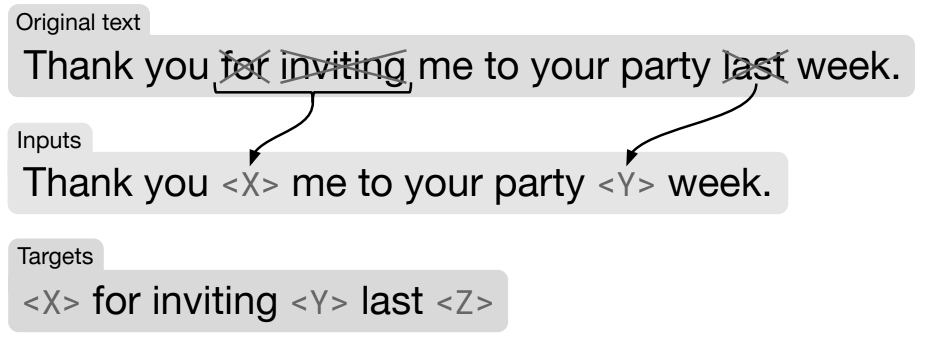
\includegraphics[width=0.6\textwidth]{pics/picard/t5-fine.png}
    \caption{Pre-training by Replace Corrupted Spans \cite{raffel_exploring_2020}}
\end{figure}

Google T5's basic idea is that it models every NLP problem and every text problem as a text-to-text task that takes the text as input and produces text as output.

So fundamentally, it is in a sequence-to-sequence framework; hence, T5 is perfectly suitable for transfer learning machine translation.
T5 can handle various tasks, and it can be fine-tuned for different NLP tasks, such as summarization, \ac{COLA}, classification, multiple text translation, also regression problems like STSB  that predict how similar two sentences are. And in our case Text-to-SQL.

\begin{figure}[H]
    \centering
    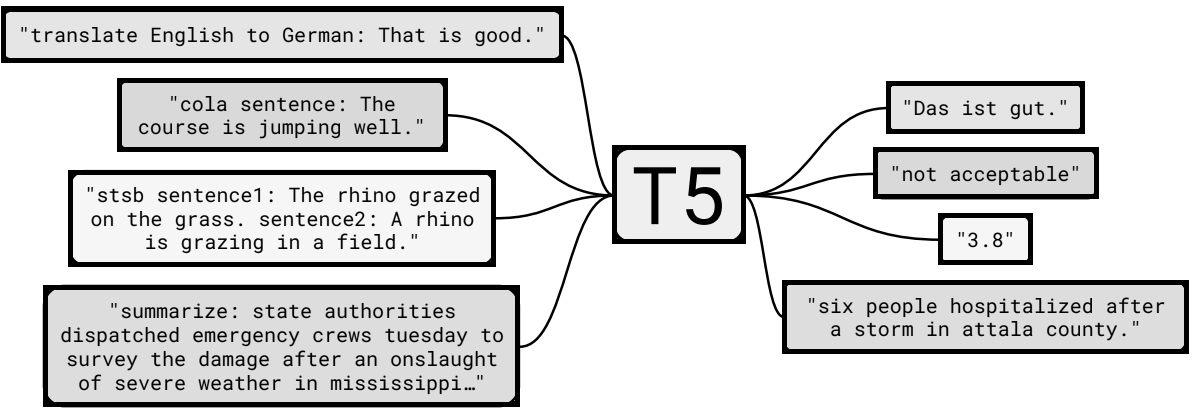
\includegraphics[width=0.9\textwidth]{pics/picard/t5-task.png}
    \caption{Each task uses text as input in the model and generates target text. In this way, the same model, loss function, and hyper-parameters are used across various diverse tasks, including translation. \cite{raffel_exploring_2020}}
\end{figure}

Further, because the same model is used for many tasks, the model understands which tasks to perform by prepending a prefix that will also be text.
Therefore, By the end of fine-tuning, T5 will have "n" different models where "n" is the number of tasks. It starts with the same base pre-trained model, and then it is fine-tuned on task A, and then separately, on task B and task C. In our work, we are essentially adding another task to the T5 to handle SQL translation.

\subsubsection*{\ac{C4}}

The T5 model is pre-trained on C4 Dataset\cite{raffel_exploring_2020}, so its results are quite realistic.
The C4 is an unlabeled dataset gathered and filtered from Common Crawl Dataset, a non-commercial crawler that saves snapshots of the web every month. And web content is dumped out on the order of 20 terabytes.

The cleaning process included deduplication, discarding incomplete sentences, and removing offensive or noisy content. The filtering led to more reliable results on downstream tasks, and the added size let the model size grow without over-fitting when pre-training. C4 is about 750 gigabytes of clean-ish data and is accessible in Tensorflow Datasets Library.


\subsubsection{Beam Search}
Before understanding the PICARD, let us first understand the concept of Beam Search:

\begin{figure}[h]
    \centering
    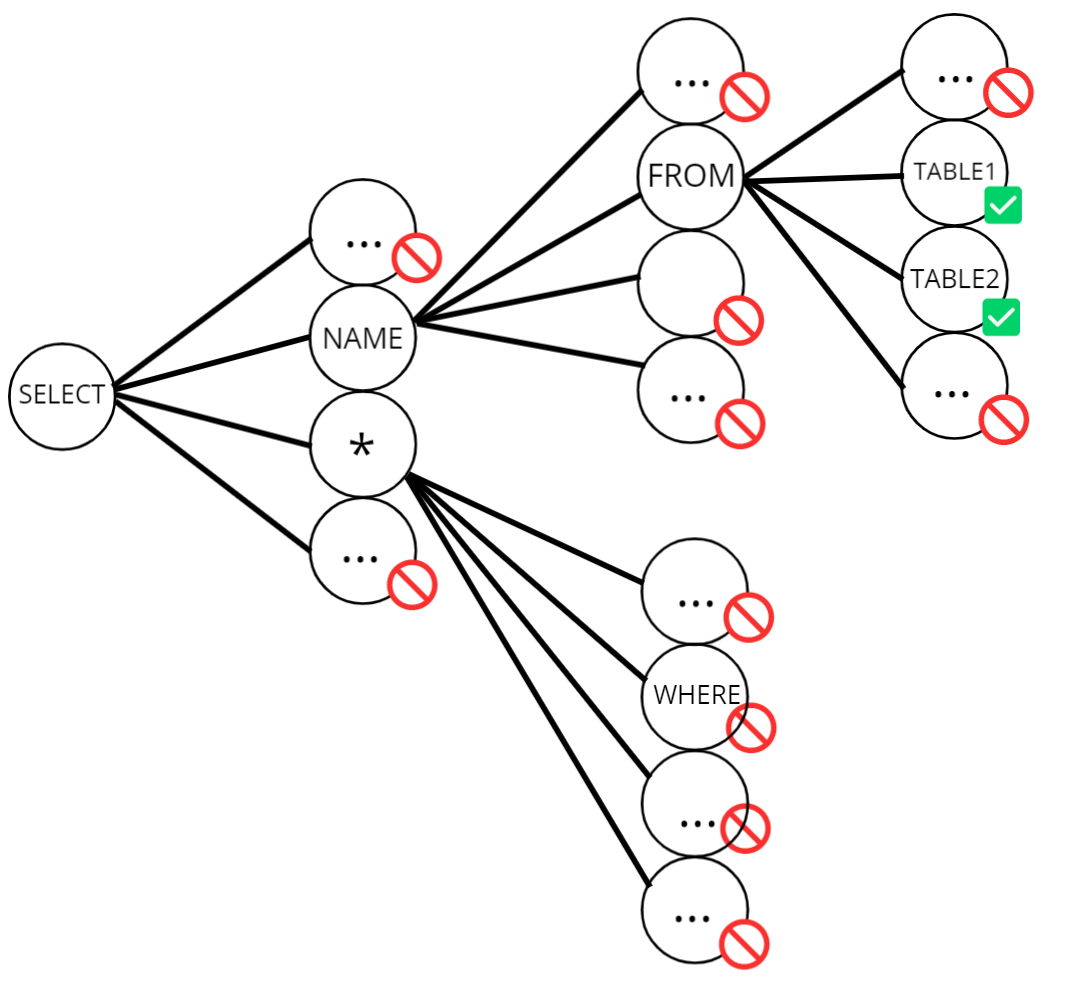
\includegraphics[width=0.8\textwidth]{pics/picard/beam.png}
    \caption{Beam Search}
    \label{fig:beam_search}
\end{figure}

Beam search is a widely used search algorithm in natural language processing and machine learning. It is beneficial in sequence-to-sequence (seq2seq) models, which generate output sequences based on input sequences. Beam search is used to find the most likely sequence of output words given an input sequence.
\\
The basic idea behind beam search is to maintain a set of the most likely sequences at each step of the decoding process. This set of sequences, called the "beam," is initially set to the starting point of the decoding process, and at each step, new sequences are generated by considering all the following possible words. The new sequences are then ranked based on their likelihood, and the highest-ranking sequences are added to the beam. The process is repeated until a stopping criterion is met \cite{10.1371/journal.pone.0211558}.
Beam search is handy in seq2seq models because it allows the model to generate multiple output sequences rather than just a single sequence. This is important because, in many cases, there may be multiple valid outputs for a given input sequence. By generating multiple outputs, beam search allows the model to explore the space of possible outputs and find the most likely sequences.
\\
One of the critical advantages of beam search is that it is computationally efficient. Because it only considers a small number of sequences at each step, it can quickly find the most likely sequences without exploring the entire space of possible outputs. This makes it well-suited for use in applications with limited computational resources, such as on mobile devices or in real-time systems.
Another advantage of beam search is that it can be used with other techniques, such as attention mechanisms, to improve the performance of seq2seq models. Attention mechanisms allow the model to focus on specific parts of the input sequence when generating the output, which can help to improve the quality of the generated sequences.
\\
In conclusion, Beam Search is a robust algorithm widely used in natural language processing and machine learning, particularly in the context of sequence-to-sequence (seq2seq) models. It allows the model to generate multiple output sequences rather than just a single sequence and is computationally efficient, making it well-suited for use in applications where computational resources are limited. Additionally, it can be combined with other techniques, such as attention mechanisms, to improve the performance of seq2seq models.

\subsubsection{PICARD}

% PICARD\cite{Scholak2021:PICARD} stands for "Parsing Incrementally for Constrained Auto-Regressive Decoding.". It can be used with any existing language model decoder or vocabulary based on auto-regressive language modeling.

% PICARD allows for the generation of executable code by constraining the output of the language model to be syntactically and semantically correct. It does this by integrating with standard beam search, a technique used in natural language processing to generate a sequence of words or tokens by expanding a beam of hypotheses step by step. At each decoding step, PICARD checks whether the most likely tokens are valid and if not, it discards them. PICARD is compatible with any model that generates a sequence of tokens and can be used with character, subword, and word-level language models without requiring exceptional recovery.

PICARD\cite{Scholak2021:PICARD}, short for "Parsing Incrementally for Constrained Auto-Regressive Decoding," is a method that can be used in conjunction with any language model decoder or vocabulary that utilizes auto-regressive language modeling.

PICARD is a technique that utilizes standard beam search, commonly used in natural language processing, to generate executable code by ensuring the output of the language model is both syntactically and semantically correct. It works by expanding a beam of hypotheses step by step and discarding any tokens that are not valid at each decoding step. This method can be applied to any language model that generates a sequence of tokens, including character, subword, and word-level models, without requiring unique recovery methods.

It effectively improves the performance of existing models and achieves state-of-the-art performance on tasks such as text-to-SQL translation.
Warps model prediction scores and integrates trivially with existing greedy and beam search algorithms used in auto-regressive decoding from language models.

At each generation step, Picard first restricts prediction to the top-k highest probability tokens and then assigns a score of negative infinity to those that fail Picard's numerous checks.

PICARD has four modes that control the level of comprehensiveness of its checking process: off, lexing, parsing without guards, and parsing with guards, with the latter being the most comprehensive. In lexing mode, PICARD checks if the current token is a valid keyword or identifier. In parsing guard mode, it checks if the current token is a valid keyword or identifier, a valid SQL keyword, and a valid SQL identifier.

Picard can detect spelling errors in keywords or reject table and column names that are invalid for the given SQL schema.
"Out-of-distribution compositional generalization and natural language variation" refers to the ability of a natural language processing (NLP) system to handle novel combinations of words and phrases that it has not seen before while also being able to handle variations in language usage.
Compositional generalization refers to the ability of an NLP system to understand and generate novel combinations of words and phrases by using its knowledge of the meanings and relationships of individual words and phrases. This is an essential aspect of NLP because it allows the system to understand and generate language flexibly and adaptively.

The concept of natural language variation refers to the multiple ways people can express the same ideas or concepts using natural language. This can include variations in dialect, style, or tone, which can make it difficult for NLP systems to understand and generate language accurately.

Together, out-of-distribution compositional generalization and natural language variation represent fundamental challenges in the field of NLP. They require NLP systems to handle a wide range of language input and output in order to be effective.

PICARD can be applied as an optional feature during inference but is not necessarily included in pre-training or fine-tuning, and for text-to-SQL translation, it works directly on the output of the language model. PICARD has been shown to have state-of-the-art performance on complex Spider text-to-SQL translation tasks, achieving an accuracy of 75.1\%.

Picard warps model prediction scores and integrates trivially with existing greedy and beam search algorithms. In addition to the token ids of the current hypothesis, the model's language modeling head also predicts the log-softmax scores for each vocabulary token. Additionally, Picard has access to SQL schema information, including table and column names and which column resides in which table.

Motivated by the success of Shaw et al. (2021)\cite{shaw-etal-2021-compositional}, who demonstrated that a pre-trained T5-Base or T5-3B model could effectively learn the text-to-SQL task, generalize to never-before-seen databases, and even rival the state-of-the-art methods of Choi et al. (2021)\cite{10.1162/coli_a_00403} without any modifications to the model itself, the researchers opted to use T5 as the baseline for all their experiments. The results from Shaw et al. (2021)\cite{shaw-etal-2021-compositional} suggest that T5-based models had the potential to improve the field of natural language processing significantly. Therefore, the researchers sought to take advantage of the capabilities of T5 in order to gain new insights into how natural language can be effectively utilized to solve complex tasks.